\documentclass{article}
\usepackage{hyperref}
\usepackage{graphicx}
\hypersetup{
    colorlinks,
    citecolor=black,
    filecolor=black,
    linkcolor=black,
    urlcolor=black
}
\begin{document}
\section{Subsystems}
\subsection{Notification Subsystem}
\subsubsection{Overview}
The notifications module provides notifications to system users regarding
particular system updates that a user would like to be notified about through
some medium external to the application.
\begin{flushleft}
For the class diagram we decided to use the observer design pattern which would be used to notify and update the Send Email and Send SMS classes, included in this is the strategy design pattern, such that Send Email and Send SMS inherit from Send Notification and this class is abstract. There are methods in the Send Email and Send SMS classes that allow users to be added to the user lists for the notifications to either or both of these mediums. There is also provision for more notification mediums to be added in the future and these can be attached to the Notify class. Should a notification medium be unavailable it can be detached from the Notify class until it is available. The Notify class can be called from any other module that would like to request a notification to be sent out to users.
\end{flushleft}

\subsubsection{UML Diagrams}	
\begin{figure}[h!]
  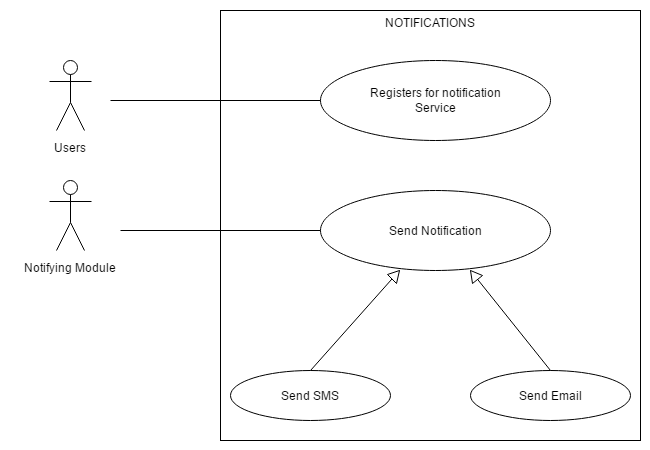
\includegraphics[width=\textwidth]{Notifications_Use_Case.png}
\end{figure}
Notification Use Case Diagram

\mbox{}\\
\bigskip


\begin{figure}[h!]
  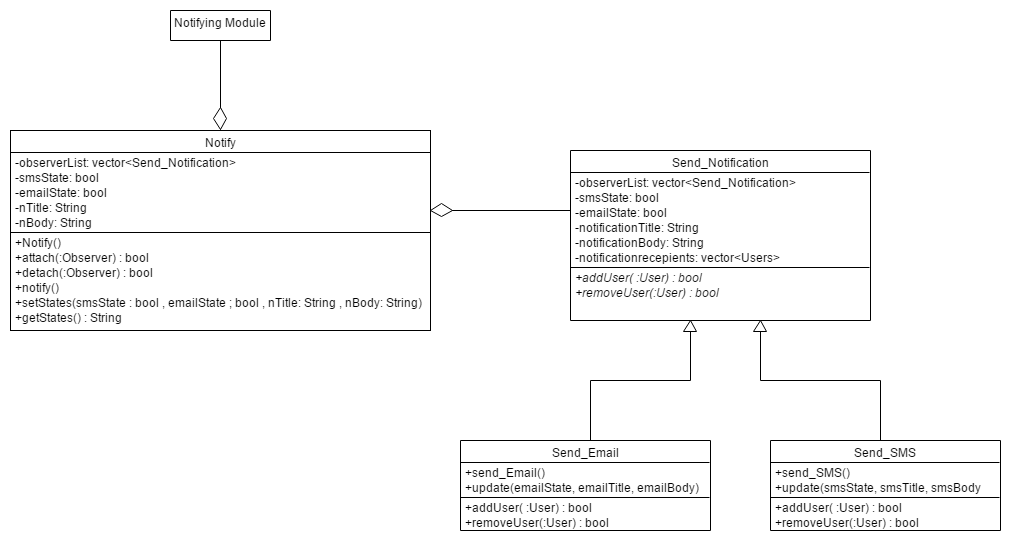
\includegraphics[width=1.3\textwidth]{Notifications_Class_Diagram.png}
\end{figure}
Notification Class Diagram

\mbox{}\\
\bigskip


\begin{figure}[h!]
  \includegraphics[width=\textwidth]{Notification_Sequence_Diagram.png}
\end{figure}
Navigation Sequence Diagram

\mbox{}\\
\bigskip
\clearpage

\begin{figure}[h!]
  \includegraphics[width=\textwidth]{Notification_Activity_Diagram.png}
\end{figure}
Navigation Activity Diagram

\mbox{}\\
\bigskip

\begin{figure}[h!]
  \includegraphics[width=0.55\textwidth]{Notification_State_Diagram.png}
\end{figure}
Navigation State Diagram

\mbox{}\\
\end{document}
